

\section{Problems and Applications}

Invariances and symmetries arise all too commonly across data originating in the real world. Hence, it should come as no surprise that some of the most popular applications of machine learning in the 21st century have come about as a direct byproduct of Geometric Deep Learning, perhaps sometimes without fully realising this fact. 
%
We would like to provide readers with an overview---by no means comprehensive---of influential works in Geometric Deep Learning and exciting and promising new applications. Our motivation is twofold: to demonstrate specific instances of scientific and industrial problems where the five geometric domains commonly arise, and to serve additional motivation for further study of Geometric Deep Learning principles and architectures.



\paragraph{Chemistry and Drug Design} One of the most promising applications of representation learning on graphs is in computational chemistry and \emph{drug development}.\marginnote{Many drugs are not designed but discovered, often serendipitously. The historic source of a number of drugs from the plant kingdom is reflected in their names: e.g., %ephedrine takes its name from the plant genus {\em Ephedra}, atropine from the belladonna plant ({\em Atropa belladonna}), and 
the acetylsalicylic acid, commonly known as {\em aspirin}, is contained in the bark of the willow tree ({\em Salix alba}), whose medicinal properties are known since antiquity.
} 
%
Traditional drugs are small molecules that are designed
to chemically attach (`bind') to some target molecule, typically a protein, in order to activate or disrupt some disease-related chemical process. 
%
Unfortunately, drug development is an extremely long and expensive process: 
at the time of writing, 
bringing a new drug to the market typically takes more than a decade and costs more than a billion dollars. 
%
One of the reasons is the cost of testing 
where many drugs fail at different stages -- less than 5\% of candidates make it to the last stage (see e.g. \cite{gaudelet2020utilising}). 




Since the space of chemically synthesisable molecules is very large (estimated around $10^{60}$), the search for candidate molecules with the right combination of properties such as target binding affinity, low toxicity, solubility, etc. cannot be done experimentally, and {\em virtual} or {\em in silico screening} (i.e., the use of computational techniques to identify promising molecules), is employed. Machine learning techniques play an increasingly more prominent role in this task. 
%
%
A prominent example of the use of Geometric Deep Learning for virtual drug screening was recently shown by \citet{stokes2020deep} %have definitively demonstrated that this is possible: 
using a graph neural network trained to predict whether or not candidate molecules inhibit growth\marginnote{ 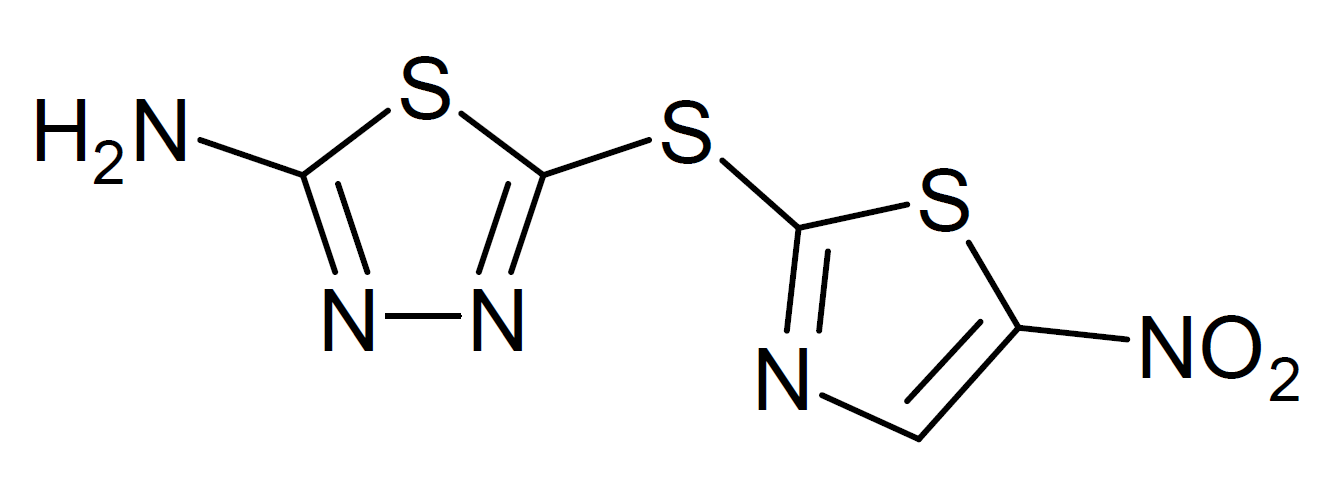
\includegraphics[width=\linewidth]{figures/Halicin_structure.png}\\ Molecular graph of Halicin.} in the model bacterium \emph{Escherichia coli}, they were able to effectively discover that \emph{Halicin}, a molecule originally indicated for treating diabetes, is a highly potent antibiotic, even against bacteria strains with known antibiotic resistance.  This discovery was widely covered in both scientific and popular press. 


Speaking more broadly, the application of graph neural networks to molecules modeled as graphs has been a very active field, with multiple specialised architectures proposed recently that are inspired by physics and e.g. incorporate equivariance to rotations and translations (see e.g. \cite{thomas2018tensor,anderson2019cormorant,fuchs2020se,satorras2021n}). Further, \citet{bapst2020unveiling} have successfully demonstrated the utility of GNNs for predictively modelling the dynamics of glass, in a manner that outperformed the previously available physics-based models.
%
Historically, many works in computational chemistry were precursors of modern graph neural network architectures sharing many common traits with them. 




\paragraph{Drug Repositioning} 
%
%\marginnote}---being able to detect novel therapeutics for existing or emerging diseases---commonly by analysing the candidate drug's molecular graph. 
While generating entirely novel drug candidates is a potentially viable approach, a faster and cheaper avenue for developing new therapies is \emph{drug repositioning}, which seeks to evaluate already-approved drugs (either alone or in combinations) for a novel purpose. 
%
This often significantly decreases the amount of clinical evaluation that is necessary to release the drug to the market. %
At some level of abstraction, the action of drugs on the body biochemistry and their interactions between each other and other biomolecules can be modeled as a graph, giving rise to the concept of `network medicine' coined by the prominent network scientist Albert-L{\'a}szl{\'o} Barab{\'a}si and advocating the use of biological networks (such as protein-protein interactions and metabolic pathways) to develop new therapies \citep{barabasi2011network}. 


Geometric Deep Learning offers a modern take on this class of  approaches. A prominent early example is the work of \cite{zitnik2018modeling}, who used graph neural networks to predict side effects in a form of drug repositioning known as {\em combinatorial therapy} or {\em polypharmacy}, formulated as edge prediction in a drug-drug interaction graph. 
%
The novel coronavirus pandemic, which is largely ongoing at the time of writing this text, has sparked a particular interest in %detecting novel therapeutics; see, e.g., 
attempting to apply such approaches against COVID-19 \citep{gysi2020network}.
%
Finally, we should note that drug repositioning is not necessarily limited to synthetic molecules: \cite{veselkov2019hyperfoods} applied similar approaches to drug-like molecules contained in food (since, as we mentioned, many plant-based foods contain biological analogues of compounds used in oncological therapy). 
%
One of the authors of this text is involved in a collaboration adding a creative twist to this research, by partnering with a molecular chef that designs exciting recipes based on the  `hyperfood' ingredients rich in such drug-like molecules. 


\paragraph{Protein biology} 
Since we have already mentioned proteins as drug targets, lets us spend a few more moments on this topic. 
%
Proteins are arguably among the most important biomolecules 
%often called the ``molecules of life'', as we are currently not aware of any life-form that is not protein-based. Proteins are encoded in our DNA and 
that have myriads of functions in our body, including protection against pathogens (antibodies), giving structure to our skin (collagen), transporting oxygen to cells (haemoglobin), catalysing chemical reactions (enzymes), and signaling (many hormones are proteins). 
%
Chemically speaking, a protein is a biopolymer, or a chain of small building blocks called {\em aminoacids} that under the influence of electrostatic forces fold into a complex 3D structure. It is this structure that endows the protein with its functions,\marginnote{A common metaphor, dating back to the chemistry Nobel laureate Emil Fischer is the {\em Schl{\"u}ssel-Schloss-Prinzip} (`key-lock principle', 1894): two proteins often only interact if they have geometrically and chemically complementary structures. } and hence it is crucial to the understanding of how proteins work and what they do. Since proteins are common targets for drug therapies, %(typical drugs are small molecules designed to bind to their target), 
the pharmaceutical industry has a keen interest in this field.

%\michael{Put AlphaFold here? }

A typical hierarchy of problems in protein bioinformatics is going from protein {\em sequence} (a 1D string over an alphabet of of 20 different amino acids) to 3D {\em structure} (a problem known as `protein folding') to {\em function} (`protein function prediction'). 
%
Recent approaches such as DeepMind's AlphaFold by  \cite{senior2020improved} used {\em contact graphs} to represent the protein structure. \cite{gligorijevic2020structure} showed that applying graph neural networks on such graphs allows to achieve better function prediction than using purely sequence-based methods. 


\cite{gainza2020deciphering} developed\marginnote{ 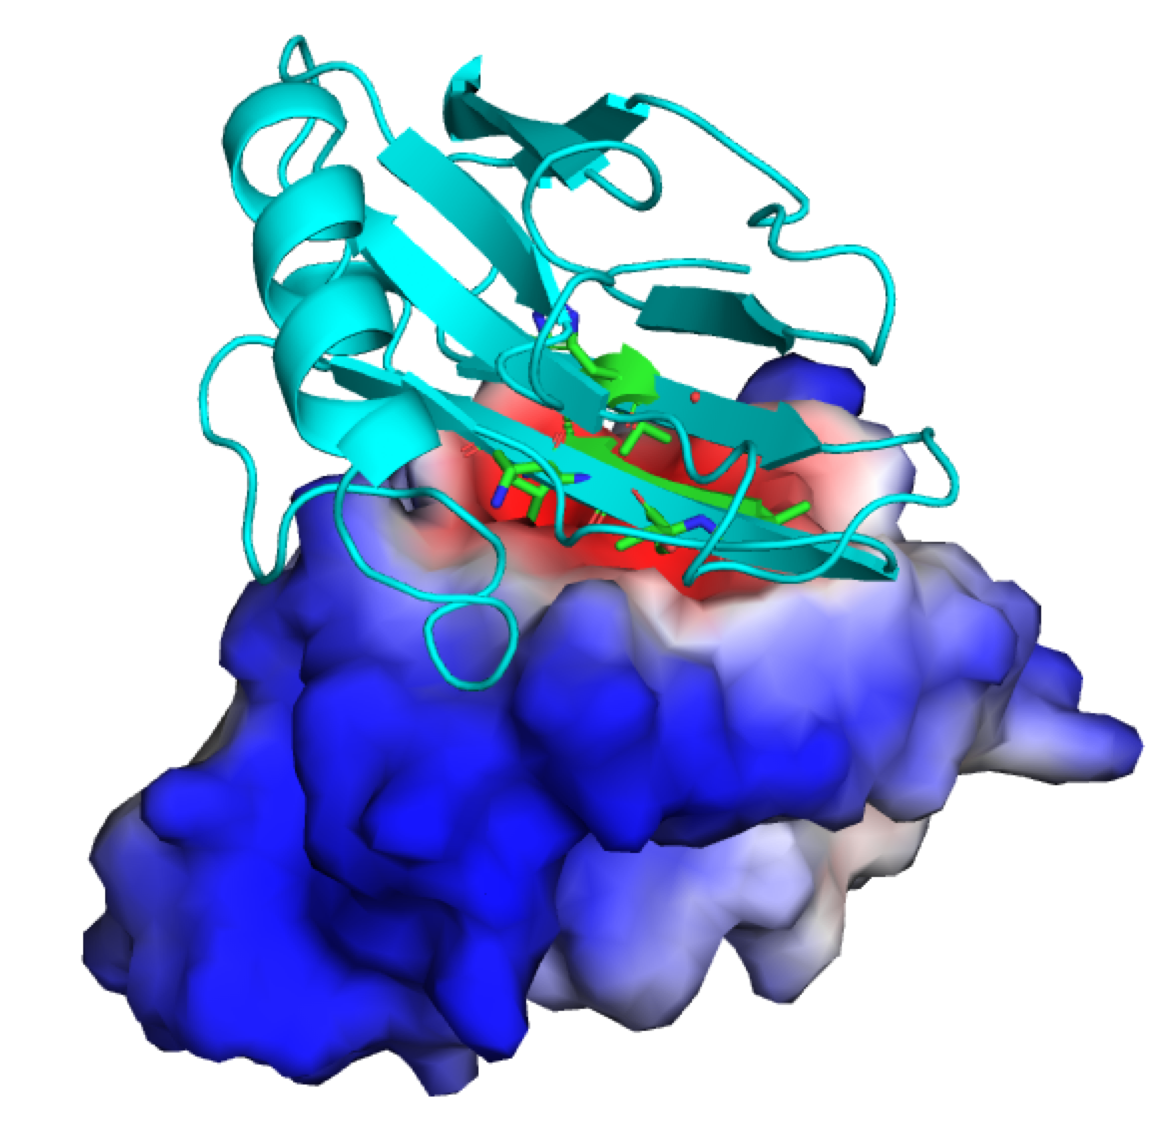
\includegraphics[width=\linewidth]{figures/masif.png}\\ Oncologial target PD-L1 protein surface (heat map indicated the predicted binding site) and the designed binder (shown as ribbon diagram).} a Geometric Deep Learning pipeline called MaSIF predicting interactions between proteins from their 3D structure. MaSIF models the protein as a molecular surface discretised as a mesh, arguing that this representation is advantageous when dealing with interactions as it allows to abstract the internal fold structure. The architecture was based on mesh convolutional neural network operating on pre-computed chemical and geometric features in small local geodesic patches. %
The network was trained using a few thousand co-crystal protein 3D structures from the Protein Data Bank to address multiple tasks, including interface prediction, ligand classification, and docking, and allowed to do {\em de novo} (`from scratch') design of proteins that could in principle act as biological immunotherapy drug against cancer -- such proteins are designed to inhibit protein-protein interactions (PPI) between parts of the programmed cell death protein complex (PD-1/PD-L1) and give the immune system the ability to attack the tumor cells.%showing state-of-the-art performance. 

%A key difference of MaSIF compared to other methods is that it does not rely on the evolutionary history of proteins. This is of crucial importance in de novo protein design, where one tries to create “from scratch” new proteins that have never existed before.



\paragraph{Recommender Systems and Social Networks} The first popularised large-scale applications of graph representation learning have occurred within \emph{social networks}\marginnote{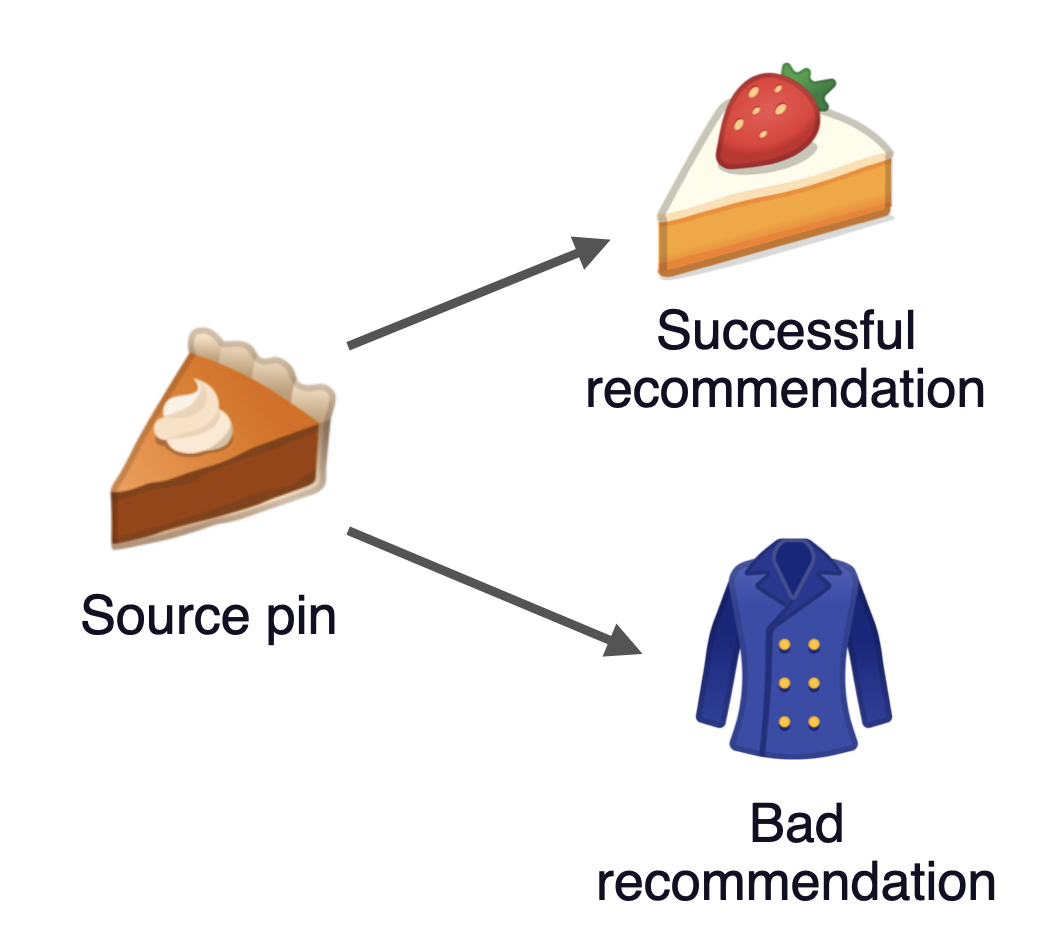
\includegraphics[width=\linewidth]{figures/Recommender.png}}, primarily in the context of \emph{recommender systems}. Recommenders are tasked with deciding which content to serve to users, potentially depending on their previous history of interactions on the service. This is typically realised through a \emph{link prediction} objective: supervise the embeddings of various nodes (pieces of content) such that they are kept close together if they are deemed \emph{related} (e.g. commonly viewed together). Then the \emph{proximity} of two embeddings (e.g. their inner product) can be interpreted as the probability that they are linked by an edge in the content graph, and hence for any content queried by users, one approach could serve its $k$ nearest neighbours in the embedding space.

Among the pioneers of this methodology is the American image sharing and social media company Pinterest: besides presenting one of the first successful deployments of GNNs in production, their method, PinSage\marginnote{Pinterest had also presented follow-up work, PinnerSage \citep{pal2020pinnersage}, which effectively integrates user-specific contextual information into the recommender.}, successfully made graph representation learning \emph{scalable} to graphs of millions of nodes and billions of edges \citep{ying2018graph}. Related applications, particularly in the space of product recommendations, soon followed. Popular GNN-backed recommenders that are currently deployed in production include Alibaba's Aligraph \citep{zhu2019aligraph} and Amazon's P-Companion \citep{hao2020p}. In this way, graph deep  learning is influencing millions of people on a daily level.


Within the context of content analysis on social networks, another noteworthy effort is Fabula AI, which is among the first GNN-based startups to be acquired (in 2019, by Twitter). The startup, founded by one of the authors of the text and his team, developed novel technology for detecting misinformation on social networks \citep{monti2019fake}. Fabula's solution consists of modelling the spread of a particular news item by the network of users who shared it. The users are connected if one of them re-shared the information from the other, but also if they follow each other on the social network. This graph is then fed into a graph neural network, which classifies the entire graph as either `true' or `fake' content -- with labels based on agreement between fact-checking bodies. Besides demonstrating strong predictive power which stabilises quickly (often within a few hours of the news spreading), analysing the embeddings of individual user nodes revealed clear clustering of users who tend to share incorrect information, exemplifying the well-known \emph{`echo chamber'} effect.

\paragraph{Traffic forecasting} Transportation networks are another area\marginnote{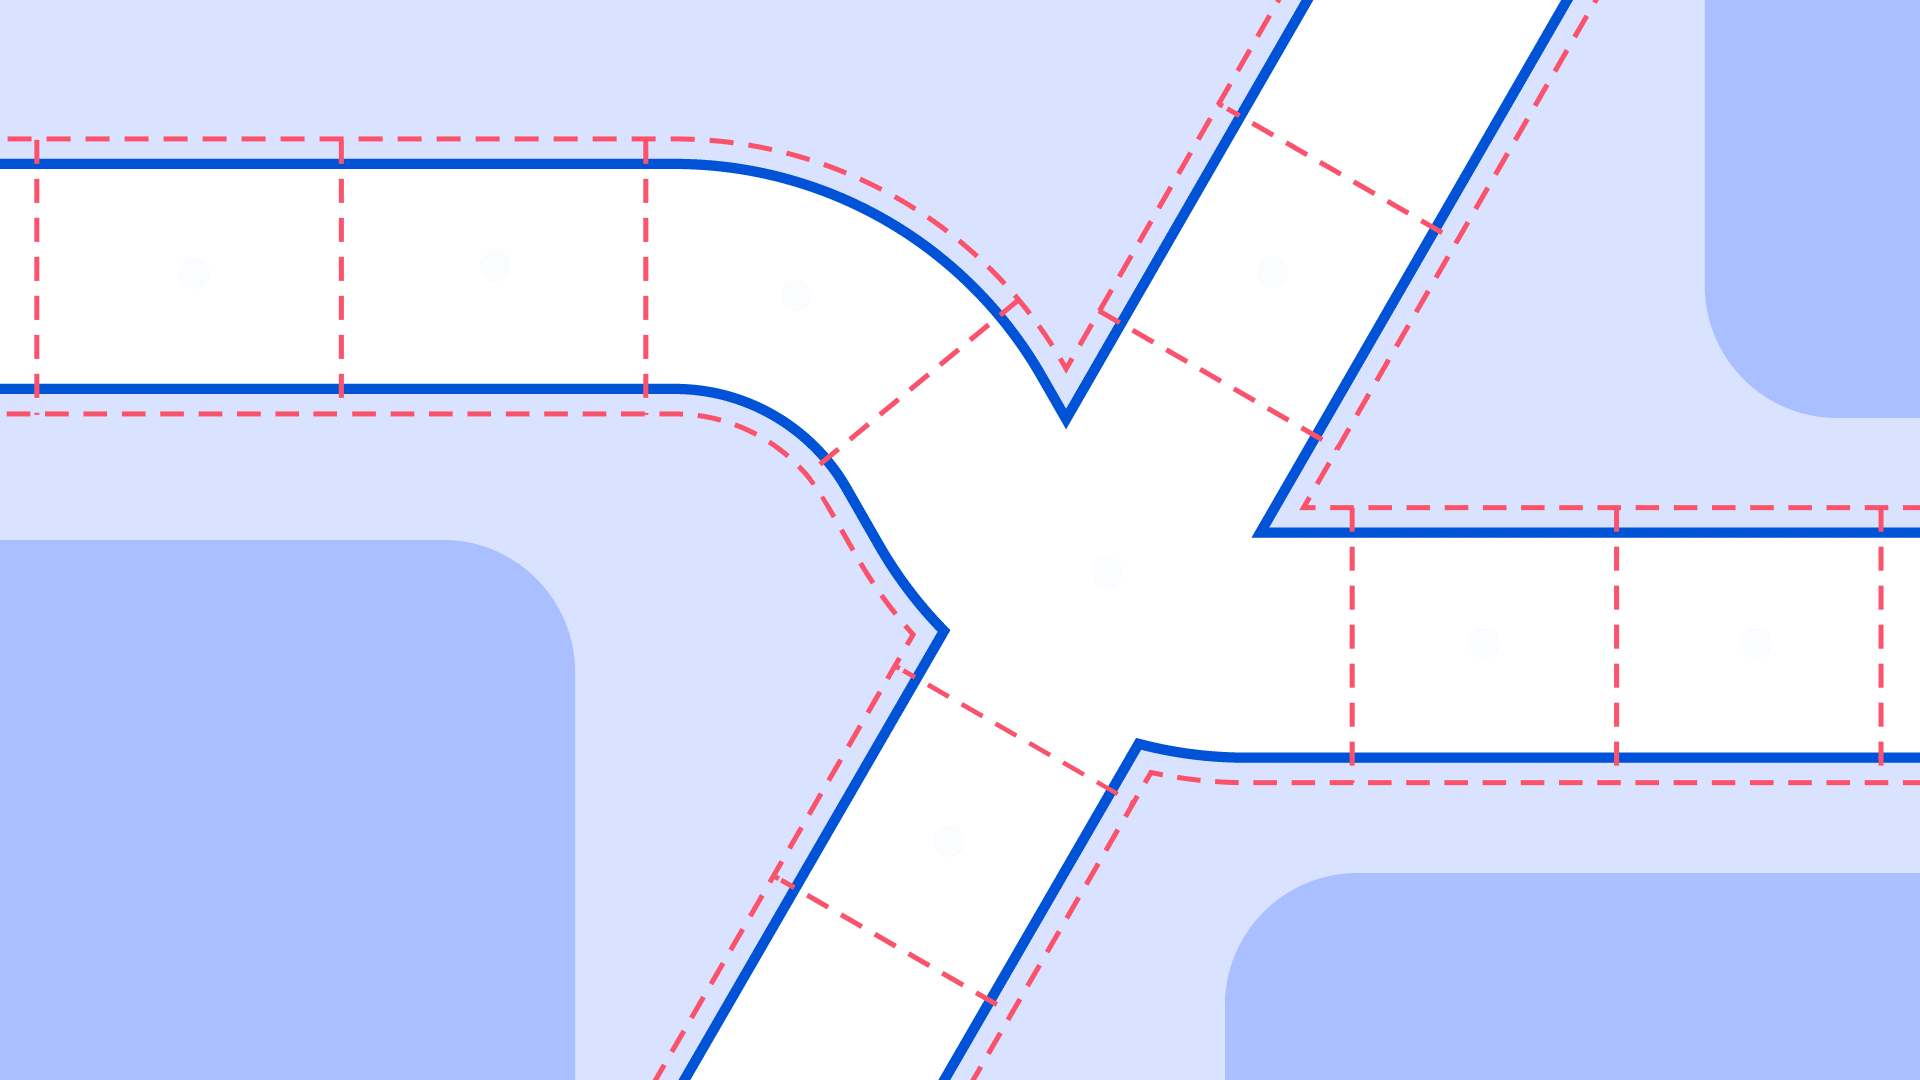
\includegraphics[width=\linewidth]{figures/superseg-1.png}\\ 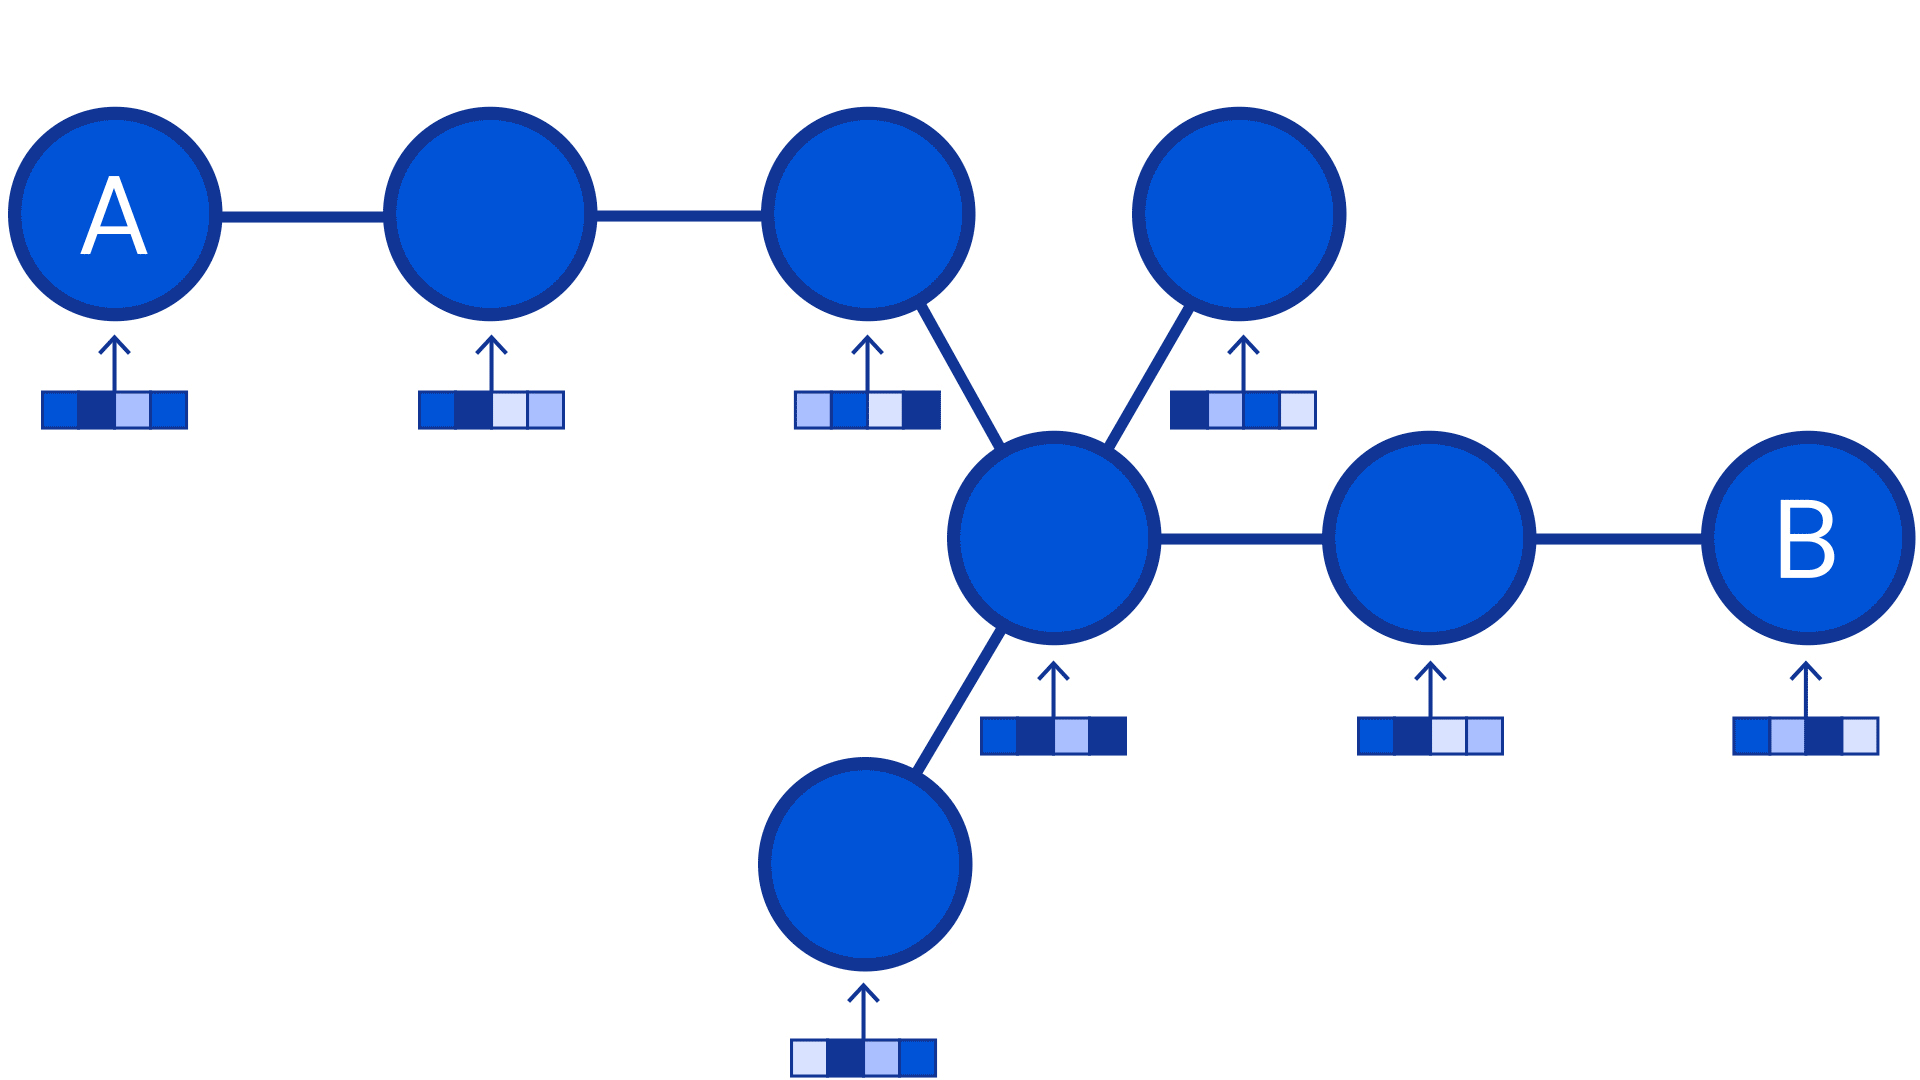
\includegraphics[width=\linewidth]{figures/superseg-3.png}\\ A road network (top) with its corresponding graph representation (bottom).} where Geometric Deep Learning techniques are already making an actionable impact over billions of users worldwide. For example, on road networks, we can observe intersections as nodes, and road segments as edges connecting them---these edges can then be featurised by the road length, current or historical speeds along their segment, and the like. 

One standard prediction problem in this space is predicting the \emph{estimated time of arrival} (ETA): for a given candidate route, providing the expected travel time necessary to traverse it. Such a problem is essential in this space, not only for user-facing traffic recommendation apps, but also for enterprises (such as food delivery or ride-sharing services) that leverage these predictions within their own operations.

Graph neural networks\marginnote{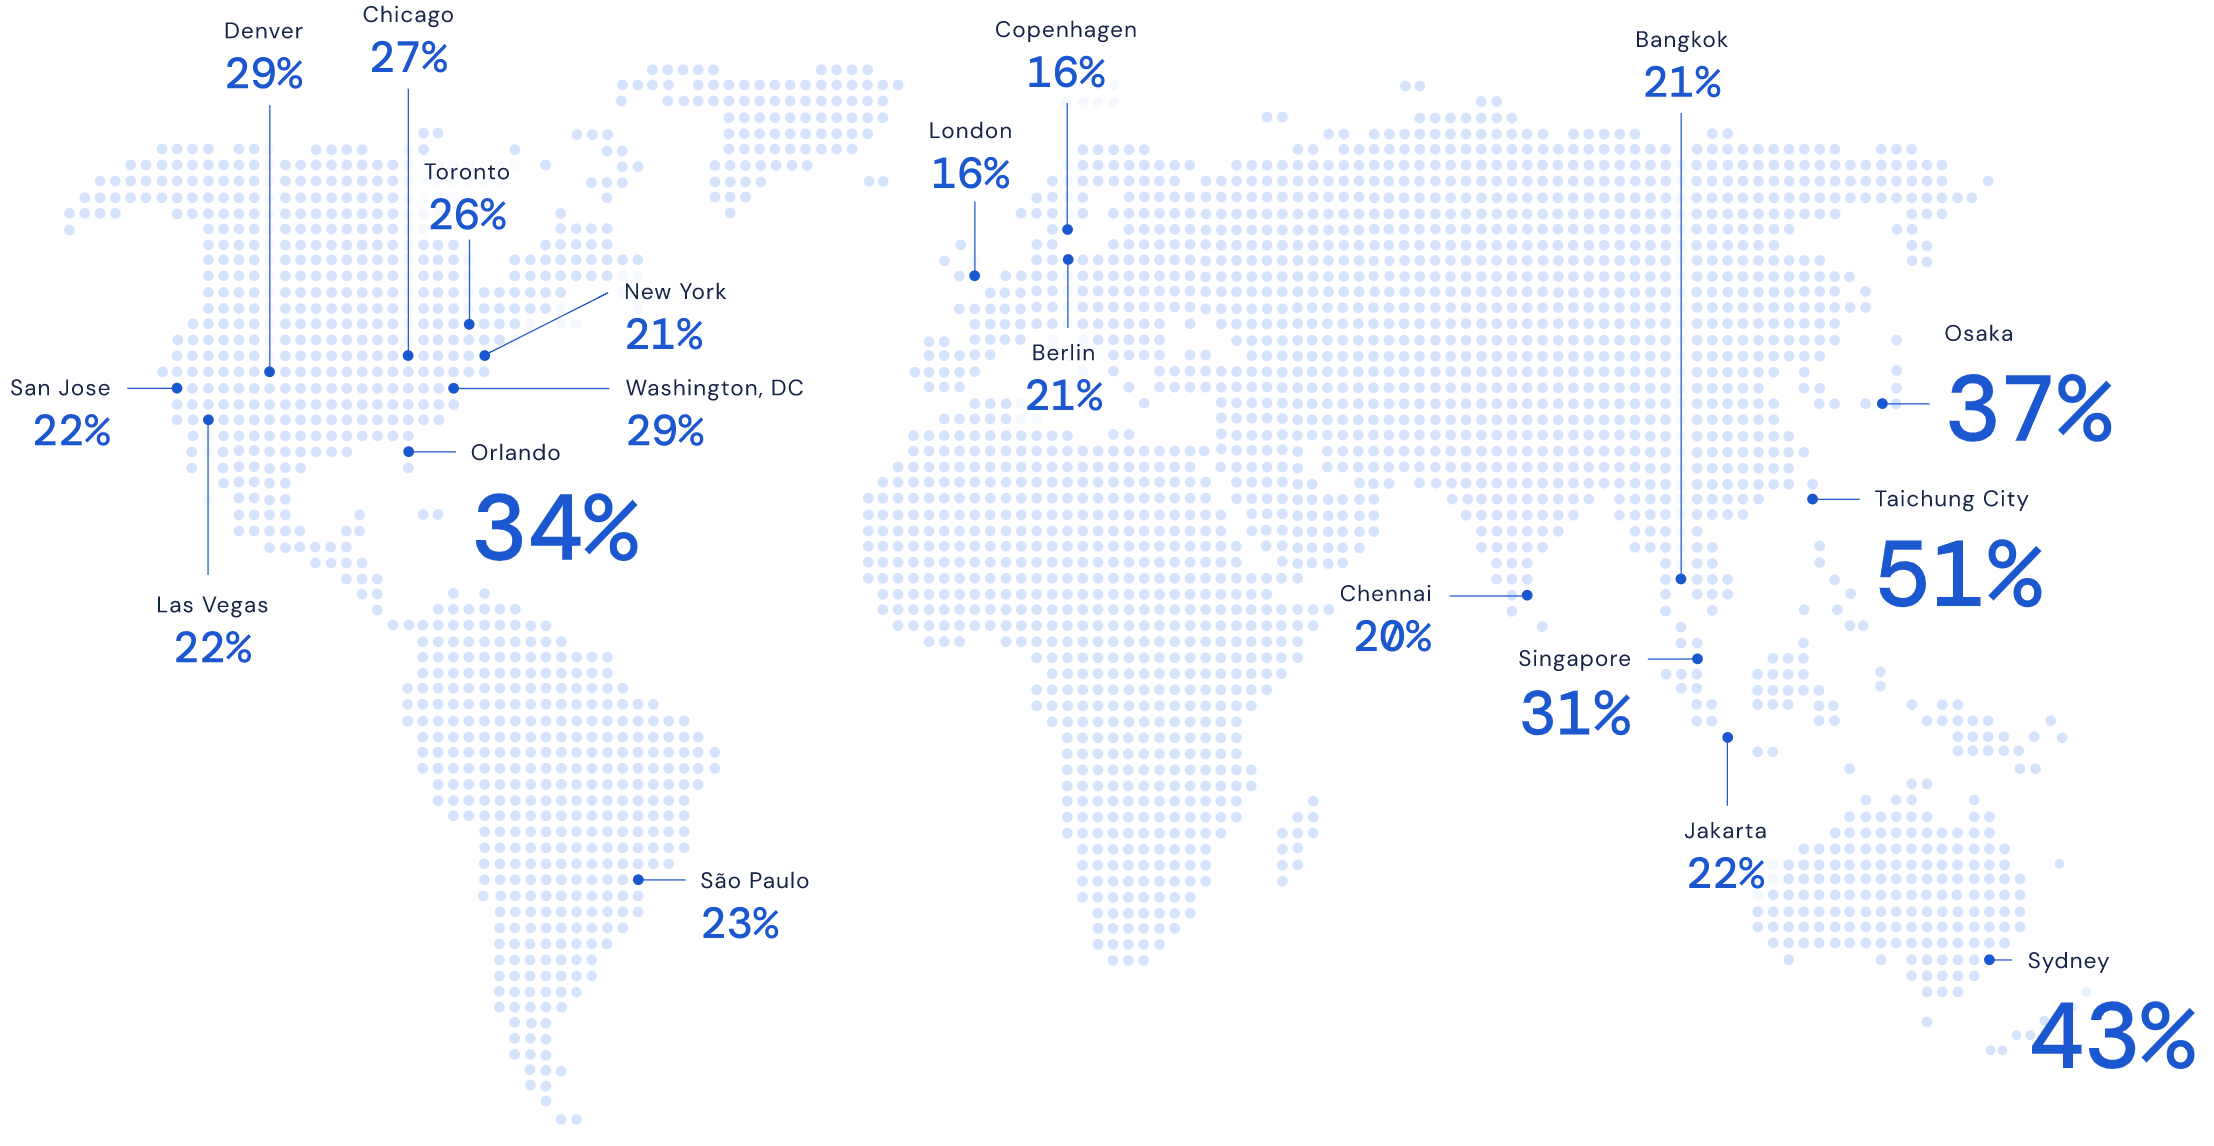
\includegraphics[width=\linewidth]{figures/maps-improvements.png}\\ Several of the metropolitan areas where GNNs are serving queries within Google Maps, with indicated relative improvements in prediction quality (40+\% in cities like Sydney).} have shown immense promise in this space as well: they can, for example, be used to directly predict the ETA for a relevant subgraph of the road network (effectively, a \emph{graph regression} task). Such an approach was successfully leveraged by DeepMind, yielding a GNN-based ETA predictor which is now deployed in production at Google Maps \citep{derrowpinion2021traffic}, serving ETA queries in several major metropolitan areas worldwide. Similar returns have been observed by the Baidu Maps team, where travel time predictions are currently served by the ConSTGAT model, which is itself based on a spatio-temporal variant of the graph attention network model \citep{fang2020constgat}.

\paragraph{Object recognition} A principal benchmark for machine learning\marginnote{
\includegraphics[width=\linewidth]{figures/tabby_cat.jpg}\\ One example input image, the likes of which can be found in ImageNet, representing the \emph{``tabby cat''} class.} techniques in computer vision is the ability to \emph{classify} a central object within a provided image. The ImageNet large scale visual recognition challenge \citep[ILSVRC]{russakovsky2015imagenet} was an annual object classification challenge that propelled much of the early development in Geometric Deep Learning. ImageNet requires models to classify realistic images scraped from the Web into one of 1000 categories: such categories are at the same time diverse (covering both animate and inanimate objects), and specific (with many classes focused on distinguishing various cat and dog breeds). Hence, good performance on ImageNet often implies a solid level of feature extraction from general photographs, which formed a foundation for various \emph{transfer learning} setups from pre-trained ImageNet models.

The success of convolutional neural networks on ImageNet---particularly the AlexNet model of \citet{krizhevsky2012imagenet}, which swept ILSVRC 2012 by a large margin---has in a large way spearheaded the adoption of deep learning as a whole, both in academia and in industry. Since then, CNNs have consistently ranked on top of the ILSVRC, spawning many popular architectures such as VGG-16 \citep{simonyan2014very}\marginnote{Interestingly, the VGG-16 architecture has sixteen convolutional layers and is denoted as ``very deep'' by the authors. Subsequent developments quickly scaled up such models to hundreds or even thousands of layers.}, Inception \citep{szegedy2015going} and ResNets \citep{he2016deep}, which have successfully surpassed human-level performance on this task. The design decisions and regularisation techniques employed by these architectures (such as rectified linear activations \citep{nair2010rectified}, dropout \citep{srivastava2014dropout}, skip connections \citep{he2016deep} and batch normalisation \citep{ioffe2015batch}) form the backbone of many of the effective CNN models in use today.

Concurrently with object classification, significant progress had been made on object \emph{detection}; that is, isolating all objects of interest within an image, and tagging them with certain classes. Such a task is relevant in a variety of downstream problems, from image captioning all the way to autonomous vehicles. It necessitates a more fine-grained approach, as the predictions need to be \emph{localised}; as such, often, translation equivariant models have proven their worth in this domain. One impactful example in this space includes the R-CNN family of models \citep{girshick2014rich,girshick2015fast,ren2015faster,he2017mask} whereas, in the related field of \emph{semantic segmentation}, the SegNet model of \citet{badrinarayanan2017segnet} proved influential, with its encoder-decoder architecture relying on the VGG-16 backbone.

\paragraph{Game playing} Convolutional neural networks also play a prominent role as translation-invariant feature extractors in \emph{reinforcement learning} (RL) environments, whenever the observed state can be represented in a grid domain; e.g. this is the case when learning to play video games from pixels. %\marginnote{\includegraphics[width=0.9\linewidth]{figures/mspacman.png} The \emph{Atari 2600} is an example of a video gaming system that has been heavily repurposed as an RL environment (primarily by the efforts of \citet{bellemare2013arcade}. Shown above is an image of \emph{Ms. Pacman}, one of the games supported therein.}.
%
In this case, the CNN is responsible for reducing the input to a flat vector representation, which is then used for deriving {\em policy} or {\em value functions} that drive the RL agent's behaviour. While the specifics of reinforcement learning are not the focus of this section, we do note that some of the most impactful results of deep learning in the past decade have come about through CNN-backed reinforcement learning.

One particular example that is certainly worth mentioning here is DeepMind's \emph{AlphaGo} \citep{silver2016mastering}. It encodes the current state within a game of Go by applying a CNN to the $19\times 19$ grid representing the current positions of the placed stones. Then, through a combination of learning from previous expert moves, Monte Carlo tree search, and self-play, it had successfully reached a level of Go mastery that was sufficient to outperform Lee Sedol, one of the strongest Go players of all time, in a five-round challenge match that was widely publicised worldwide. 

While this already represented a significant milestone for broader artificial intelligence---with Go having a substantially more complex state-space than, say, chess\marginnote{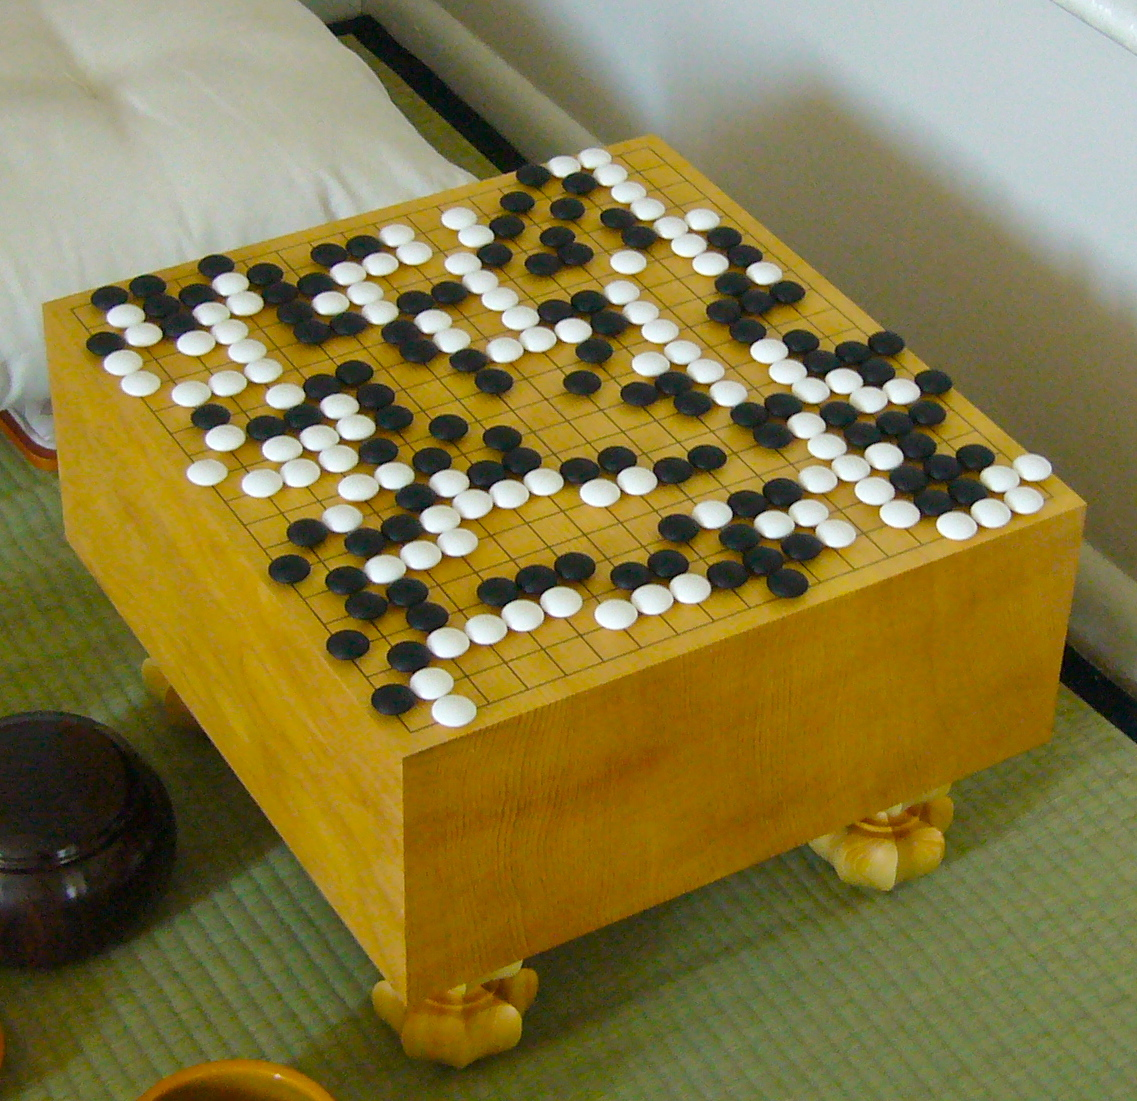
\includegraphics[width=\linewidth]{figures/Go_board.jpeg} The game of Go is played on a $19\times 19$ board, with two players placing white and black \emph{stones} on empty fields. The number of legal states has been estimated at $\approx2\times 10^{170}$ \citep{tromp2006combinatorics}, vastly outnumbering the number of atoms in the universe.}---the development of AlphaGo did not stop there. The authors gradually removed more and more Go-specific biases from the architecture, with \emph{AlphaGo Zero} removing human biases, optimising purely through self-play \citep{silver2017mastering}, \emph{AlphaZero} expands this algorithm to related two-player games, such as Chess and Shogi; lastly, \emph{MuZero} \citep{schrittwieser2020mastering} incorporates a model that enables \emph{learning} the rules of the game on-the-fly, which allows reaching strong performance in the Atari 2600 console, as well as Go, Chess and Shogi, without any upfront knowledge of the rules. Throughout all of these developments, CNNs remained the backbone behind these models' representation of the input.

While several high-performing RL agents were proposed for the Atari 2600 platform over the years \citep{mnih2015human,mnih2016asynchronous,schulman2017proximal}, for a long time they were unable to reach human-level performance on \emph{all} of the 57 games provided therein. This barrier was finally broken with Agent57 \citep{badia2020agent57}, which used a parametric family of policies, ranging from strongly exploratory to purely exploitative, and prioritising them in different ways during different stages of training. It, too, powers most of its computations by a CNN applied to the video game's framebuffer.

\paragraph{Text and speech synthesis} Besides images (which naturally map to a \emph{two}-dimensional grid), several of (geometric) deep learning's strongest successes have happened on one-dimensional grids. Natural examples of this are \emph{text} and \emph{speech}, folding the Geometric Deep Learning blueprint within diverse areas such as natural language processing and digital signal processing.

Some of the most widely applied and publicised works in this space focus on \emph{synthesis}: being able to generate speech or text, either unconditionally or conditioned on a particular \emph{prompt}. Such a setup can support a plethora of useful tasks, such as  \emph{text-to-speech} (TTS), predictive text completion, and machine translation. Various neural architectures for text and speech generation have been proposed over the past decade, initially mostly based on \emph{recurrent} neural networks (e.g. the aforementioned seq2seq model \citep{sutskever2014sequence} or recurrent attention \citep{bahdanau2014neural}). However, in recent times, they have been gradually replaced by convolutional neural networks and Transformer-based architectures.

One particular limitation of simple 1D convolutions in this setting is their linearly growing \emph{receptive field}, requiring many layers in order to cover the sequence generated so far. \emph{Dilated}\marginnote{Dilated convolution is also referred to as \emph{\`{a} trous} convolution (literally \emph{``holed''} in French).} convolutions, instead, offer an \emph{exponentially} growing receptive field with an equivalent number of parameters. Owing to this, they proved a very strong alternative, eventually becoming competitive with RNNs on machine translation \citep{kalchbrenner2016neural}, while drastically reducing the computational complexity, owing to their parallelisability across all input positions.\marginnote{Such techniques have also outperformed RNNs on problems as diverse as protein-protein interaction \citep{deac2019attentive}.} The most well-known application of dilated convolutions is the \emph{WaveNet} model from \cite{oord2016wavenet}. WaveNets demonstrated that, using dilations, it is possible to synthesise speech at the level of \emph{raw waveform} (typically 16,000 samples per second or more), producing speech samples that were significantly more ``human-like'' than the best previous text-to-speech (TTS) systems\marginnote{Besides this, the WaveNet model proved capable of generating piano pieces.}. Subsequently, it was further demonstrated that the computations of WaveNets can be distilled in a much simpler model, the \emph{WaveRNN} \citep{kalchbrenner2018efficient}---and this model enabled effectively deploying this technology at an industrial scale. This allowed not only its deployment for large-scale speech generation for services such as the Google Assistant, but also allowing for efficient on-device computations; e.g. for Google Duo, which uses end-to-end encryption.

Transformers \citep{vaswani2017attention} have managed to surpass the limitations of both recurrent and convolutional architectures, showing that \emph{self-attention} is sufficient for achieving state-of-the-art performance in machine translation. Subsequently, they have revolutionised natural language processing. Through the pre-trained embeddings provided by models such as BERT \citep{devlin2018bert}, Transformer computations have become enabled for a large amount of downstream applications of natural language processing---for example, Google uses BERT embeddings to power its search engine. 

Arguably the most widely publicised application of Transformers in the past years is text generation, spurred primarily by the \emph{Generative Pre-trained Transformer} (GPT, \cite{radford2018improving,radford2019language,brown2020language}) family of models from OpenAI. In particular, GPT-3 \citep{brown2020language} successfully scaled language model learning to 175 billion learnable parameters, trained on next-word prediction on web-scale amounts of scraped textual corpora. This allowed it not only to become a highly-potent few-shot learner on a variety of language-based tasks, but also a text generator with capability to produce coherent and human-sounding pieces of text. This capability not only implied a large amount of downstream applications, but also induced a vast media coverage.

\paragraph{Healthcare} 
%
Applications in the medical domain are another promising area for Geometric Deep Learning. There are multiple ways in which these methods are being used. 
%
First, more traditional architectures such as CNNs have been applied to grid-structured data, for example, for the 
prediction of length of stay in Intensive Care Units
\citep{rocheteau2020temporal}, 
or diagnosis of sight-threatening diseases from retinal scans \citep{de2018clinically}. 
%
\cite{winkels2019pulmonary} showed that using 3D roto-translation group convolutional networks improves 
the accuracy of pulmonary nodule detection compared to conventional CNNs.  


Second, modelling organs as geometric surfaces, mesh convolutional neural networks were shown to be able to address a diverse range of tasks, from reconstructing facial structure from genetics-related information \citep{mahdi20203d} to 
brain cortex parcellation \citep{cucurull2018convolutional} to 
regressing demographic properties from cortical surface structures \citep{besson2020geometric}. 
%
%The latter problems consists of []
%Third, 
%
The latter examples represent an increasing trend in  neuroscience to consider the brain as a surface with complex folds\marginnote{Such structure of the brain cortex are called {\em sulci} and {\em gyri} in anatomical literature.} giving rise to highly non-Euclidean structures. 
%since the data in this field are often represented on surface models of the brain. 
%as many cortical properties only make sense considering their specific location with respect to the various sulci and gyri [8]. These surface models are essentially sheet-like meshes that are intricately folded in three-dimensional space, maintaining the geometrical structure of the brain


At the same time, 
neuroscientists often try construct and analyse {\em functional networks} of the brain representing the various regions of the brain that are activated together when performing some cognitive function; these networks are often constructed using functional magnetic resonance imaging (fMRI) that shows in real time which areas of the brain consume more blood.\marginnote{Typically, Blood Oxygen-Level Dependent (BOLD) contrast imaging is used. } 
%
These functional networks can reveal patient demographics (e.g., telling apart males from females, \cite{arslan2018graph}), as well as used for neuropathology diagnosis, which is the third area of application of Geometric Deep Learning in medicine we would like to highlight here. In this context, \cite{ktena2017distance} pioneered the use of graph neural networks for the prediction of neurological conditions such as Autism Spectrum Disorder. 
%
The geometric and functional structure of the brain appears to be intimately related, and recently \cite{itani2021combining} pointed to the benefits of exploiting them jointly in neurological disease analysis.  
% can reveal important information about the complexity of the neuropathology


Fourth, {\em patient networks} are becoming more prominent in ML-based medical diagnosis. The rationale behind these methods is that the information of patient demographic, genotypic, and phenotypic similarity could improve predicting their disease.  
%
 \cite{parisot2018disease} 
 applied graph neural networks on networks of patients created from demographic features for neurological disease diagnosis, showing that the use of the graph improves prediction results.
 %
\cite{cosmo2020latent} showed the benefits of latent graph learning (by which the network {\em learns} an unknown patient graph) in this setting.  The latter work used data from the UK Biobank, a large-scale collection of medical data including brain imaging \citep{miller2016multimodal}. 




A wealth of data about hospital patients may be found in \emph{electronic health records} (EHRs)\marginnote{Publicly available anonymised critical-care EHR datasets include MIMIC-III \citep{johnson2016mimic} and eICU \citep{pollard2018eicu}.}. Besides giving a comprehensive view of the patient's progression, EHR analysis allows for \emph{relating} similar patients together. This aligns with the \emph{pattern recognition method}, which is commonly used in diagnostics. Therein, the clinician uses \emph{experience} to recognise a pattern of clinical characteristics, and it may be the primary method used when the clinician's experience may enable them to diagnose the condition quickly. Along these lines, several works attempt to construct a patient graph based on EHR data, either by analysing the embeddings of their doctor's notes \citep{malone2018learning}, diagnosis similarity on admission \citep{rocheteau2021predicting}, or even assuming a fully-connected graph \citep{zhu2019graph}. In all cases, promising results have been shown in favour of using graph representation learning for processing EHRs.



\paragraph{Particle physics and astrophysics} 
High energy physicists were perhaps among the first domain experts in the field of natural sciences to embrace the new shiny tool, graph neural networks. 
%
In a recent review paper, \cite{shlomi2020graph}\marginnote{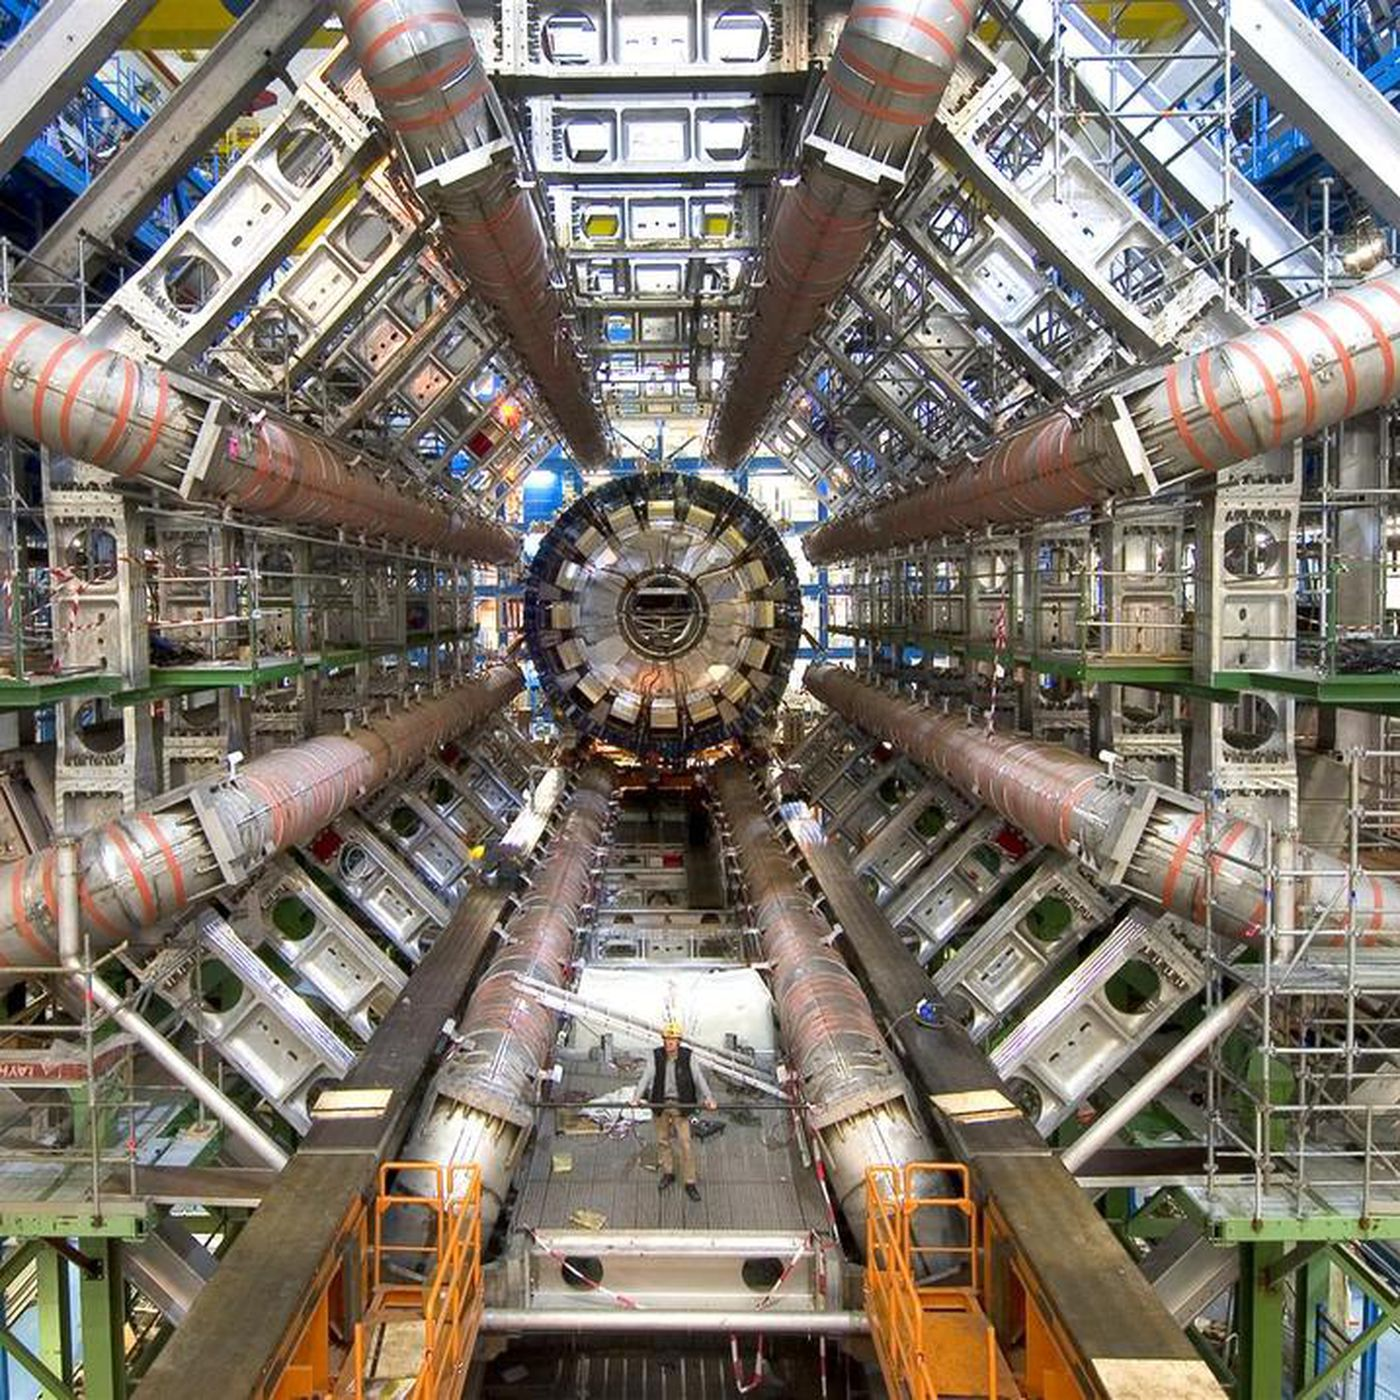
\includegraphics[width=\linewidth]{figures/lhc.jpeg} 
Part of the Large Hadron Collider detectors. 
} note that machine learning has historically been heavily used in particle physics experiments, either to learn complicated inverse functions allowing to infer the underlying physics process from the information measured in the detector, or to perform classification and regression tasks. For the latter, it was often necessary to force the data into an unnatural representation such as grid, in order to be able to used standard deep learning architectures such as CNN. Yet, many problems in physics involve data in the form of unordered sets with rich relations and interactions, which can be naturally represented as graphs. 


One important application in high-energy physics is the reconstruction and classification of {\em particle jets} -- sprays of stable particles %that are stemming 
arising from multiple successive interaction and decays of particles originating from a single
initial event. % (for example, a collision of ). 
%
In the Large Hardon Collider, the largest and best-known particle accelerator built at CERN, such jet are the result of collisions of protons at nearly the speed of light. 
%ccelerated to a speed close to that of light, they collide with other protons. 
These collisions produce massive particles, such as the long though-for Higgs boson or the top quark.  
%
%object. 
%
The identification and classification of collision events is of crucial importance, as it might provide experimental evidence to the existence of new particles.  


Multiple Geometric Deep Learning approaches\marginnote{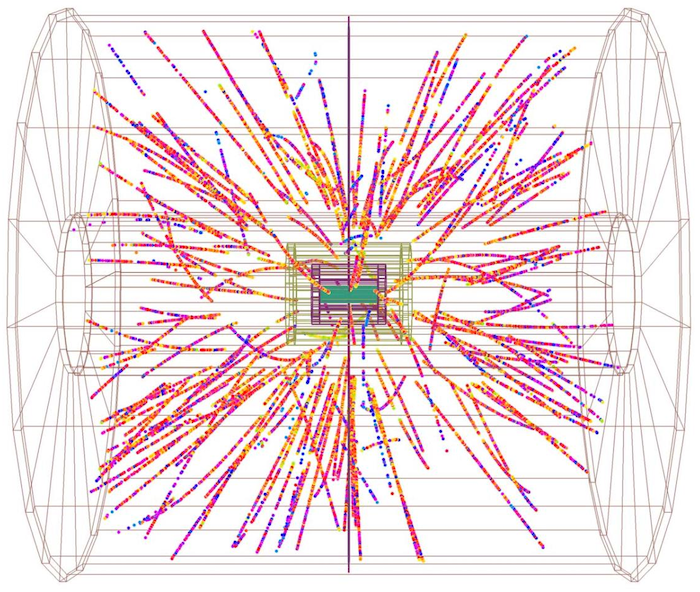
\includegraphics[width=\linewidth]{figures/particlejet.png} 
Example of a particle jet. 
} have recently been proposed for particle jet classification task, e.g. by \cite{komiske2019energy} and \cite{qu1902particlenet},  based on DeepSet and Dynamic Graph CNN architectures, respectively. 
%
%Recently GNNs have been extended by adding inductive biases
More recently, there has also been interest in developing specialsed architectures derived from physics consideration and incorporating inductive biases consistent with Hamiltonian or Lagrangian mechanics (see e.g. \cite{sanchez2019hamiltonian,cranmer2020lagrangian}), equivariant to the Lorentz group (a fundamental symmetry of space and time in physics) \citep{bogatskiy2020lorentz}, or even incorporating symbolic reasoning \citep{cranmer2019learning} and capable of learning physical laws from data. Such approaches are more interpretable (and thus considered more `trustworthy' by domain experts) and also offer better generalisation. 



Besides particle accelerators,
 particle detectors are now being used by astrophysicist for {\em multi-messenger astronomy} --  a new way of coordinated observation of disparate signals, such as electromagnetic radiation, gravitational waves, and neutrinos, coming from the same source. 
%
Neutrino astronomy is of particular interest, since neutrinos interact only very rarely with matter, and thus travel enormous distances practically unaffected.\marginnote{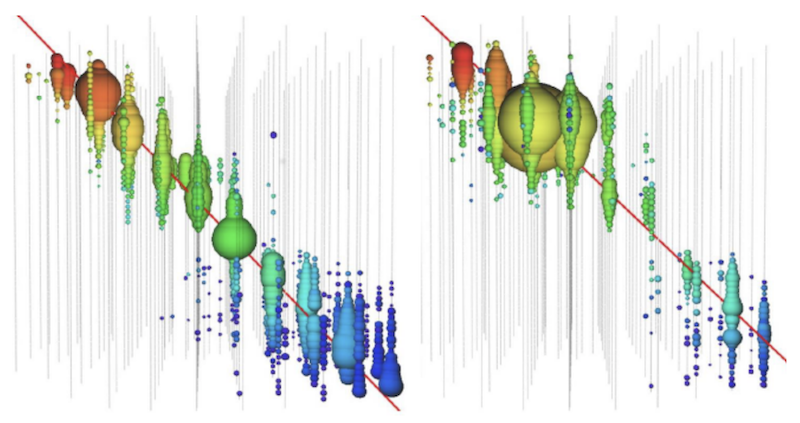
\includegraphics[width=\linewidth]{figures/icecube.png} The characteristic pattern of light deposition in IceCube detector from background events (muon bundles, left)
and astrophysical neutrinos (high-energy single muon, right). \cite{choma2018graph}
} Detecting neutrinos allows to observe objects inaccessible to optical telescopes, but requires enormously-sized detectors -- the IceCube neutrino observatory uses a cubic kilometer of Antarctic ice shelf on the South Pole as its detector. 
%
Detecting high-energy neutrinos can possibly shed lights on some of the most mysterious objects in the Universe, such as blazars and black holes. 
%
\cite{choma2018graph} used a Geometric neural network to model the irregular geometry of the IceCube neutrino detector, showing significantly better performance in detecting neutrinos coming from astrophysical sources and separating them from background events. 


While neutrino astronomy offers a big promise in the study of the Cosmos, traditional optical and radio telescopes are still the `battle horses' of astronomers. 
%
With these traditional instruments, Geometric Deep Learning can still offer new methodologies for data analysis. For example, \cite{scaife2021fanaroff} used rotationally-equivariant CNNs for the classification of radio galaxies, and \cite{mcewen2021scattering} used 
spherical CNNs for the analysis of cosmic microwave background radiation, a relic from the Big Bang that might shed light on the formation of the primordial Universe. As we already mentioned, such signals are naturally represented on the sphere and equivariant neural networks are an appropriate tool to study them. 


%\michael{TACO: anything on the sphere? There is a work of Defferard, but I don't like it because they use GNNs on the meshed sphere, which is non comme il faut}

%[47], which can improve performance and generalization on various physical
%prediction problems. Other recent work [7] has shown symbolic physical laws can be
%extracted from the learned functions within a GN.


%For additional details on various applications of Geometric Deep Learning in particle physics, we refer the reader to a recent review by \cite{shlomi2020graph}. 



\paragraph{Virtual and Augmented Reality} 
Another field of applications which served as the motivation for the development of a large class of Geometric Deep Learning methods is computer vision and graphics, in particular, dealing with 3D body models for virtual and augmented reality. 
%
Motion capture technology used to produce special effects in movies like Avatar often operates in two stages: first, the input from a 3D scanner capturing the motions of the body or the face of the actor is put into correspondence with some canonical shape, typically modelled as a discrete manifold or a mesh (this problem is often called `analysis'). Second, a new shape is generated to repeat the motion of the input (`synthesis').  
%
Initial works on Geometric Deep Learning in computer graphics and vision \citep{masci2015geodesic,boscaini2016learning,monti2017geometric} developed mesh convolutional neural networks to address the analysis problem, or more specifically, deformable shape correspondence. 


First geometric autoencoder architectures for 3D shape synthesis were proposed independently by \cite{litany2018deformable} and  \cite{ranjan2018generating}. In these architectures, a canonical mesh (of the body, face, or hand) was assumed to be known and the synthesis task consisted of regressing the 3D coordinates of the nodes (the embedding of the surface, using the jargon of differential geometry). %,bouritsas2019neural}. 
%
\cite{kulon2020weakly} showed \marginnote{ 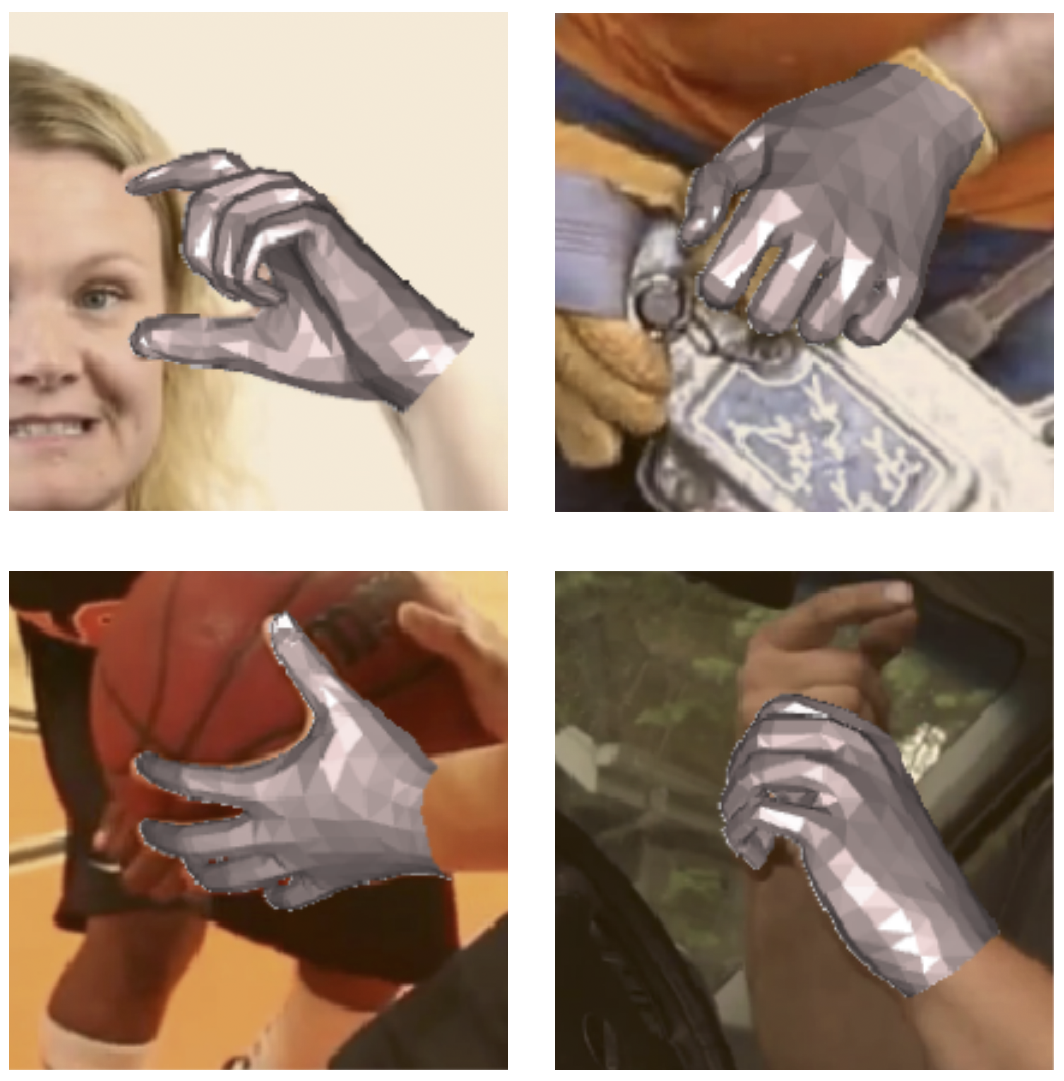
\includegraphics[width=\linewidth]{figures/ariel.png}\\ Examples of complex 3D hand poses reconstructed from 2D images in the wild \citep{kulon2020weakly}.}a hybrid pipeline for 3D hand pose estimation with an image CNN-based encoder and a geometric decoder. A demo of this system, developed in collaboration with a British startup company Ariel AI and presented at CVPR 2020, allowed to create realistic body avatars with fully articulated hands from video input on a mobile phone faster than real-time.  %
Ariel AI was acquired by Snap in 2020, and at the time of writing its technology is used in Snap's augmented reality products. 
%Shape correspondence, Protein molecular surfaces, Ariel AI